
\subsubsection{Genus a rozkład na sumę węzłów pierwszych}

\begin{proposition}
    \label{prp:genus_of_sum}
    Jeśli $J, K$ są węzłami, to $g (J \shrap K) = g(J) + g(K)$.
\end{proposition}

Poniższy dowód pochodzi od Schuberta (\cite{schubert49}), został tylko zapisany we współczesnym języku.
\index[persons]{Schubert, Horst}%
Przebiega w dwóch etapach: najpierw pokazuje się, że genus sumy nie jest większy od sumy genusów składników, a następnie, że nie jest od niej mniejszy.

\begin{proof}
    Pokażemy najpierw, że $g(J \# K) \le g(J) + g(K)$.
    Wybierzmy powierzchnie Seiferta $M_J$ oraz $M_K$ dla $J$ oraz $K$ o~minimalnym genusie.
    Suma $J \shrap K$ powstaje z~$J$ oraz $K$, podobnie jest z~powierzchniami Seiferta:
\begin{comment}
    \begin{figure}[H]
        \centering
        \begin{minipage}[b]{.48\linewidth}
        \[
            \LargeGenusProofA \longrightarrow \LargeGenusProofB
        \]
        \subcaption{suma węzłów}
        %
        \end{minipage}
        \begin{minipage}[b]{.48\linewidth}
        \[
            \LargeGenusProofC \longrightarrow \LargeGenusProofD
        \]
        \subcaption{suma powierzchni}
        \end{minipage}
    \end{figure}
\end{comment}

    Skoro $M_{J\#K}$ powstaje z~$M_J \sqcup M_K$ przez dołączenie paska do brzegu, mamy
    \begin{equation}
        \chi(M_{J\#K}) = \chi(M_J \sqcup M_K) - 1 = \chi(M_J) + \chi(M_K)-1,
    \end{equation}
    a~przez to
    \begin{equation}
        g(M_{J\#K}) = \frac{1-\chi(M_{J\#K})}{2} =
        \frac{1-\chi(M_{J})}{2} + \frac{1-\chi(M_{K})}{2}
        % = %g(M_J)+g(M_K)
        = g(J) + g(K).
    \end{equation}
    To kończy dowód pierwszej nierówności.
    Pokażemy jeszcze, że $g(J \# K) \ge g(J)+g(K)$.
    Zaczynamy od powierzchni Seiferta $M_{J\#K}$ dla $J\#K$ o~minimalnym genusie $g(M_{J\#K})$ równym $g(J\#K)$.
    Poprzez wykonanie chirurgii na powierzchni, możemy przyjąć specjalną postać jak w~poprzednim dowodzie:
\begin{comment}
    \[
        \LargeGenusProofD
    \]
\end{comment}

    Usunięcie paska daje powierzchnie Seiferta dla $M_J$ oraz $M_K$ takie, że
    \begin{equation}
        g(M_J)+g(M_K)=g(M_{J\#K})=g(J\#K).
    \end{equation}
    Oznacza to, że $g(J) + g(K) \le g(M_J) + g(M_K) = g(J\#K)$ i~mamy równość.
\end{proof}

Jesteśmy wreszcie w~stanie podać prawdziwy dowód faktu \ref{first_time_sum_is_trivial}.

\begin{corollary}
    \label{cor:connected_sum_no_inverses}
    Jeśli suma spójna dwóch węzłów jest niewęzłem, to oba składniki także nim są.
\end{corollary}

Powrócimy teraz do węzłów pierwszych.
\index{węzeł!pierwszy}%

\begin{proposition}
    Niech $K$ będzie węzłem.
    Jeśli $g(K) = 1$, to $K$ jest węzłem pierwszym.
\end{proposition}

\begin{proof}
    Załóżmy nie wprost, że węzeł $K = K_1 \# K_2$ jest sumą dwóch nietrywialnych węzłów.
    Z~faktu \ref{prp:genus_of_sum} wynika wtedy, że $g(K) = g(K_1) + g(K_2)$.
    Zatem jeden z węzłów $K_1, K_2$ ma genus zero i jest trywialny, wbrew naszemu założeniu.
\end{proof}

Implikacja odwrotna jest fałszywa: pięciolistnik jest pierwszy, ale jego genus wynosi $2$.

\begin{proposition}
    Każdy węzeł można zapisać jako suma spójna pewnej liczby węzłów pierwszych.
    Niewęzeł jest sumą pustej rodziny węzłów.
\end{proposition}

\begin{proof}
    Dowodzimy przez indukcję względem genusu $g(K)$.
    Przypadek bazowy $g(K) = 0$ jest oczywisty, gdyż wtedy $K$ to niewęzeł.
    Załóżmy więc, że fakt zachodzi dla węzłów $J$ genusu co najwyżej $n$.
    Niech $K$ będzie genusu $n + 1$.

    Jeśli $K$ jest pierwszy, nie ma czego dowodzić.
    W przeciwnym razie jest równoważny z~$J_1 \shrap J_2$, gdzie $J_1$ i~$J_2$ są nietrywialne.
    Mamy $g(J_1) + g(J_2) = g(K)$ oraz $g(J_1),g(J_2) \ge 1$.
    Zatem $g(J_1), g(J_2) \le n$.
    Na mocy hipotezy indukcyjnej, $J_1$ oraz $J_2$ są równoważne sumom
    \[
        J_1 \cong K_1\#\cdots\# K_s,\qquad
        J_2 \cong K_{s+1}\#\cdots\# K_r,
    \]
    gdzie $K_i$ są pierwsze.
    Zatem $K$ jest równoważny z~$K_1\#\cdots\# K_r$, co kończy dowód.
\end{proof}

Nasz aparat matematyczny jest niedostatecznie rozwinięty, by móc udowodnić jedyność rozkładu.

\begin{theorem}[Schubert, 1949]
    Każdy nietrywialny węzeł rozkłada się na węzły pierwsze.
    Rozkład jest, z dokładnością do kolejności składników, jednoznaczny.
\index{węzeł!pierwszy}%
\end{theorem}

Schubert podał geometryczny dowód oparty o powierzchnie Seiferta; wyraził go w języku PL-rozmaitości (\cite{schubert49}), ale niedużym wysiłkiem można dokonać adaptacji do gładkiego świata.
\index[persons]{Schubert, Horst}%
Praca Schuberta korzysta z twierdzenia Alexandera, że 2-sfera w przestrzeni $\R^3$ ogranicza dysk, i jego odpowiednika dla torusów w $S^3$.

Hashizume \cite{hashizume58} rozszeszył wyniki Schuberta do splotów.
\index[persons]{Hashizume, Yoko}%
% trzeba wspomnieć, że to wymaga adaptacji definicji sumy spójnej, bo wcześniej dopuszczaliśmy tylko węzły jako składniki. Remedium = Kawauchi.

\begin{proposition}
    \label{prp:infinitely_many_prime_knots}
    Istnieje nieskończenie wiele węzłów pierwszych.
\end{proposition}

\begin{proof}
    Pokażemy, że wszystkie węzły $(2n+2)_1$ są pierwsze, gdzie $n \ge 1$.
    Istotnie, algorytm Seiferta zastosowany do diagramu tego węzła wyprodukuje $2n+1$ okręgów.
\begin{comment}
    \[
        \begin{tikzpicture}[baseline=-0.65ex,scale=0.06]
        \begin{knot}[clip width=7, flip crossing/.list={1,4,5},end tolerance=1pt]
            \node at (0,10) {$\cdots$};
            \strand[semithick] (-30, -5) -- (-5, -5);
            \strand[semithick]  (5, -5) -- (30, -5);
            \strand[semithick,latex-]  (-30,-15) -- (-5,-15);
            \strand[semithick]  (5,-15) -- (30,-15);

            \strand[semithick] (-5, -15) [in=down, out=right] to (5, -10) [in=right, out=up] to (-5, -5);
            \strand[semithick] (5, -15) [in=down, out=left] to (-5, -10) [in=left, out=up] to (5, -5);

            % zewnętrzne obręcze -- lewa strona
            \strand[semithick] (-30, 15) to [out=left, in=up]   (-45, 0);
            \strand[semithick] (-30,-15) to [out=left, in=down] (-45, 0);
            \strand[semithick] (-30,  5) to [out=left, in=up]   (-35, 0);
            \strand[semithick] (-30, -5) to [out=left, in=down] (-35, 0);

            % zewnętrzne obręcze -- prawastrona
            \strand[semithick] (30, 15) to [out=right, in=up]   (45,0);
            \strand[semithick] (30,-15) to [out=right, in=down] (45,0);
            \strand[semithick] (30,  5) to [out=right, in=up]   (35,0);
            \strand[semithick] (30, -5) to [out=right, in=down] (35,0);

            % jak w~drugim ruchu Reidemeistera - górny warkocz, lewy
            \strand[semithick] (-30, 15) [in=left, out=right] to (-20,  5);
            \strand[semithick] (-30,  5) [in=left, out=right] to (-20, 15);
            \strand[semithick] (-10, 15) [in=right, out=left] to (-20,  5);
            \strand[semithick] (-10,  5) [in=right, out=left] to (-20, 15);

            % jak w~drugim ruchu Reidemeistera - górny warkocz, prawy
            \strand[semithick] (30, 15) [in=right, out=left] to (20,  5);
            \strand[semithick] (10, 15) [in=left, out=right] to (20,  5);
            \strand[semithick] (30,  5) [in=right, out=left] to (20, 15);
            \strand[semithick] (10,  5) [in=left, out=right] to (20, 15);
        \end{knot}
        \end{tikzpicture}
        \longrightarrow
        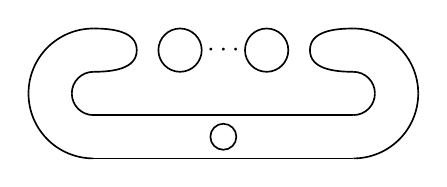
\begin{tikzpicture}[baseline=-0.65ex,scale=0.055]
            \node at (0,10) {$\cdots$};
            \draw[semithick] (-30,  -5) -- (30, -5);
            \draw[semithick] (-30, -15) -- (30,-15);

            \draw[semithick] (0,-10) circle (3);

                % zewnętrzne obręcze -- lewa strona
            \draw[semithick] (-30, 15) to [out=left, in=up]   (-45, 0);
            \draw[semithick] (-30,-15) to [out=left, in=down] (-45, 0);
            \draw[semithick] (-30,  5) to [out=left, in=up]   (-35, 0);
            \draw[semithick] (-30, -5) to [out=left, in=down] (-35, 0);

                % zewnętrzne obręcze -- prawastrona
            \draw[semithick] (30, 15) to [out=right, in=up]   (45,0);
            \draw[semithick] (30,-15) to [out=right, in=down] (45,0);
            \draw[semithick] (30,  5) to [out=right, in=up]   (35,0);
            \draw[semithick] (30, -5) to [out=right, in=down] (35,0);

            \draw[semithick] (-30, 15) to [out=right, in=up] (-20,10);
            \draw[semithick] (-30,  5) to [out=right, in=down] (-20,10);

            \draw[semithick] (30, 15) to [out=left, in=up] (20,10);
            \draw[semithick] (30,  5) to [out=left, in=down] (20,10);

            \draw[semithick] (-10, 10) circle (5);
            \draw[semithick] (10,  10) circle (5);
        \end{tikzpicture}
    \]
\end{comment}
    Wynika stąd, że genus wynosi $\frac 12 (1 - (1+2n) + (2+2n)) = 1$, ponieważ wyznacznik ma wartość $4n+1$,
    węzły $(2n+2)_1$ nie są trywialne i~są parami różne.
\end{proof}

